\documentclass[12pt]{article}
\usepackage{minted}
\usepackage{multirow}
\usepackage{listings}
\usepackage{amssymb,amsmath,amsthm,amsfonts}
\usepackage{graphicx}
\usepackage{titlesec}
\usepackage{gensymb}
\usepackage{url}
\usepackage{fancyhdr}
\usepackage[spanish]{babel}
\usepackage[nolist]{acronym}
\usepackage[table]{xcolor}
\usepackage{url}
\usepackage{float}
\usepackage{parskip}

% HYPERLINK CONFIGURATION %
\usepackage[colorlinks=true, allcolors=blue]{hyperref}
\hypersetup{
    colorlinks=true,% make the links colored
}
    
% MARGINS CONFIGURATION %
\usepackage{vmargin}
\setmarginsrb{2 cm}{2 cm}{2 cm}{2 cm}{1 cm}{1.5 cm}{1 cm}{1.5 cm}

% GRAPHICS CONFIGURATION %
\usepackage{graphicx}
\graphicspath{{images/}}

\begin{document}

\begin{titlepage}

    \title{     \textbf{Propuesta de Tesis de Grado \\ de Ingeniería en Informática}\\[2.5ex]
        \textit{Detección de Deadlocks en Rust \\en tiempo de compilación \\mediante Redes de Petri} }

    \author{
        \textbf{Director:} Ing. Pablo A. Deymonnaz\\[2.5ex]
        \textbf{Alumno:} Horacio Lisdero Scaffino, \textit{(Padrón \# 100.132)}                                \\
        \texttt{ hlisdero@fi.uba.ar }                                    \\[2.5ex]
        \normalsize{Facultad de Ingeniería, Universidad de Buenos Aires}        \\
    }

    \date{6 de marzo de 2023}

\end{titlepage}

\maketitle
\thispagestyle{empty}

\maketitle{
    \hypersetup{linkcolor=black}
    \tableofcontents
}

\section{Introducción}

\subsection{El problema de la correctitud en programación concurrente}

En el área de computación concurrente, uno de los desafíos principales es probar la correctitud de un programa concurrente.
A diferencia de un programa secuencial donde para cada entrada se obtiene siempre la misma salida, en un programa concurrente
la salida puede depender de cómo se intercalaron las instrucciones de los diferentes procesos o hilos durante la ejecución.

La correctitud de un programa concurrente se define entonces en términos de propiedades del cómputo realizado y no solamente en términos del
resultado obtenido. En la bibliografía \cite{ben-ari2006, coulouris2012, tanenbaum2017} se definen dos tipos de propiedades de correctitud:

\begin{itemize}
    \item Propiedades de \textit{safety}: Propiedades que se deben cumplir \textit{siempre}.
    \item Propiedades de \textit{liveness}: Propiedades que se deben cumplir \textit{eventualmente}.
\end{itemize}

Dos de las propiedades de tipo \textit{safety} deseables en un programa concurrente son:

\begin{itemize}
    \item \textbf{Exclusión mutua}: dos procesos no deben acceder a recursos compartidos al mismo tiempo.
    \item \textbf{Ausencia de \textit{deadlock}}: un sistema en ejecución debe poder continuar realizando su tarea, es decir, avanzar produciendo trabajo útil.
\end{itemize}

Usualmente se utilizan primitivas de sincronización tales como mutexes, semáforos, monitores y \textit{condition variables}
para implementar el acceso coordinado de los procesos o hilos a los recursos compartidos.
No obstante, el uso correcto de estas primitivas es difícil de lograr en la práctica y se pueden introducir errores difíciles de detectar y corregir.
Actualmente la mayoría de lenguajes de uso general, ya sean compilados o interpretados, no permiten detectar estos errores en todos los casos.

Dada la creciente importancia de la programación concurrente debida a la proliferación de sistemas de hardware multihilo y multiproceso,
reducir el número de \textit{bugs} ligados a la sincronización de los procesos o hilos es de vital importancia para la industria.
Evitar los \textit{deadlocks} es un requerimiento ineludible en el desarrollo,
especialmente en sistemas embebidos y sistemas de misión crítica como vehículos autónomos o aeronaves.

\subsection{Redes de Petri}

Las redes de Petri son una herramienta gráfica y matemática ampliamente utilizada para describir sistemas distribuidos,
introducidas por el investigador alemán Carl Adam Petri en su tesis de doctorado \cite{petri1962}.
Un resumen conciso de la teoría de redes de Petri, sus propiedades, análisis y aplicaciones se encuentra en \cite{murata1989}.

Una red de Petri consiste en un grafo dirigido bipartito, el cual cuenta con dos tipos de nodos: lugares (\textit{places}) y transiciones (\textit{transitions}).
Únicamente pueden existir arcos dirigidos entre un lugar y una transición o entre una transición y un lugar.
A los lugares se les asignan marcas (\textit{tokens}) los cuales representan el estado actual del sistema o un recurso en particular.

\begin{figure}[H]
    \centering
    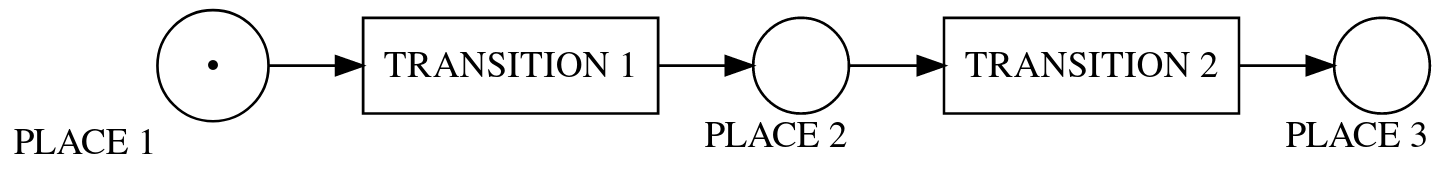
\includegraphics[scale=0.25]{petri-net-example.png}
    \caption{Ejemplo de una red de Petri. \texttt{PLACE 1} contiene un \textit{token}.}
\end{figure}

Las transiciones se disparan siguiendo la siguiente regla:
\begin{itemize}
    \item Se consume un \textit{token} de los lugares cuyos arcos entran a la transición.
    \item Se crea un token en cada lugar al cual llega un arco saliente de la transición.
\end{itemize}

\begin{figure}[H]
    \centering
    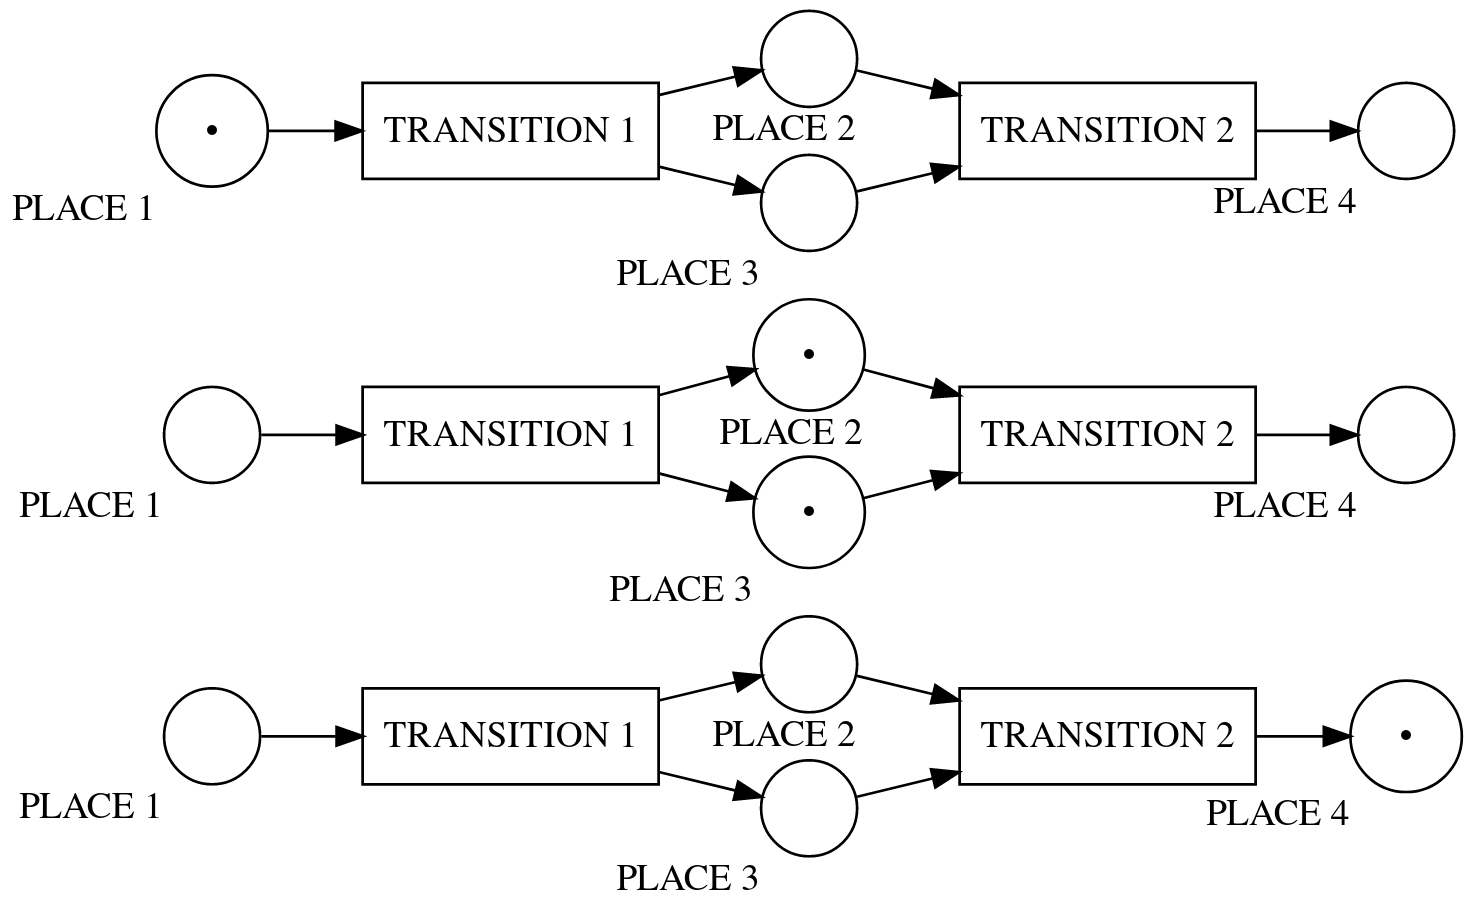
\includegraphics[scale=0.25]{petri-net-transition-firing-example.png}
    \caption{Ejemplo de disparo de transiciones. Primero se dispara la transición 1 y luego la transición 2.}
\end{figure}

Las redes de Petri pueden ser vistas como una versión generalizada de las máquinas de estado que permite modelar la concurrencia y el paralelismo.
Su uso como método formal de validación de software está establecido desde finales de los años 1980 y
existen redes de Petri que permiten modelar primitivas de sincronización como enviar un mensaje o esperar a la recepción de un mensaje \cite{heiner1998}.
Se pueden utilizar también para validar requerimientos de software expresados mediante casos de uso \cite{silva-dossantos2004},
para modelar procesos industriales \cite{aalst1994} o para especificar y analizar sistemas de tiempo real \cite{kavi2011}.

Existen varias técnicas que permiten encontrar \textit{deadlocks} en una red de Petri.
El método más conocido se denomina análisis de alcance (\textit{reachability analysis}) \cite{murata1989}.
En este se construye un grafo dirigido que representa los estados posibles que la red de Petri puede alcanzar durante su ejecución.
En este grafo cada nodo representa un estado posible de la red y cada arista representa una transición que permite pasar de un estado al otro.
Se puede demostrar matemáticamente que la existencia de un nodo sin aristas salientes implica la existencia de un \textit{deadlock} en la red de Petri.

La desventaja de este análisis es su elevado costo computacional, el cual crece de forma exponencial
con la cantidad de nodos de la red de Petri cuando no se puede hacer uso de hipótesis o heurísticas adicionales.
La complejidad computacional del llamado \textit{reachability problem} es de hecho NP-completo para ciertas clases de redes de Petri.
Sin embargo, existen clases de redes para las cuales la complejidad es menor, incluso polinomial.
En \cite{esparza1994} se detallan los resultados teóricos más importantes obtenidos hasta 1998.

Además existen métodos alternativos para detección de \textit{deadlocks}
como el método basado en sifones (una estructura específica que ocurre en muchas redes de Petri) \cite{hu2011} y
el método basado en jerarquías de abstracción \cite{kungas2005}.
En particular, este último autor propone un método muy prometedor de orden polinomial para evitar el problema
de la explosión de estados que subyace al algoritmo \textit{naïve} de detección de \textit{deadlocks}.
A través de un algoritmo que abstrae una red de Petri dada a una representación más simple,
se obtiene una jerarquía de redes de tamaño creciente para las cuales la verificación de ausencia de \textit{deadlocks} resulta sustancialmente más rápida.
Es, dicho de una forma burda, una estrategia del tipo ``divide y vencerás'' que verifica la ausencia de \textit{deadlocks}
en partes de la red para luego ir construyendo la verificación del todo final agregando partes a la red pequeña inicial.

\subsection{Motivación}
\label{motivation}

En el presente trabajo nos proponemos estudiar la detección de \textit{deadlocks} y \textit{lost signals} en el lenguaje de programación Rust.
Se utilizará un modelo teórico basado en redes de Petri para encontrar los errores en el código fuente.
Mediante una traducción del código fuente en tiempo de compilación,
se obtendrá una red de Petri que luego podrá ser analizada mediante métodos de verificación de modelos para garantizar la ausencia de \textit{deadlocks}.

El objetivo es contribuir a la comunidad de Rust aportando una primera versión de esta herramienta que podría luego ser extendida para soportar casos más complejos.
Se busca que el uso de la herramienta sea lo más sencillo y accesible posible para fomentar su uso y aplicación a proyectos reales de software.
Por esta razón la tesis contará con una primera implementación del traductor que podrá ser utilizado como \textit{plugin}
del gestor de paquetes estándar de Rust \textit{cargo}\footnote{\url{https://doc.rust-lang.org/stable/cargo/}}.

A largo plazo se podría incorporar la herramienta al compilador como un pase adicional opcional en el proceso de compilación.
Este pase verificaría que no se pueden producir ciertas clases de \textit{deadlocks}, lo que haría de Rust un lenguaje de programación aún más seguro y confiable.

Con el propósito de que el trabajo pueda ser leído por el mayor número de personas posible y
que forme parte de la documentación de los respectivos repositorios de código publicados en GitHub,
resulta imprescindible redactar el manuscrito en idioma inglés.

Por otra parte, nos proponemos implementar una funcionalidad de exportado de la red de Petri obtenida a partir del código fuente
a formatos estandarizados a fin de facilitar la interoperabilidad con otras herramientas de verificación de modelos y visualización de redes de Petri.
Como parte de la investigación previa se encontró que dos formatos son particularmente relevantes en este sentido:

\begin{itemize}
    \item DOT\footnote{\url{https://graphviz.org/}}: un lenguaje de visualización de gráficos de código abierto, parte de la suite Graphviz \cite{dot2015}.
    \item Petri Net Markup Language (PNML)\footnote{\url{https://www.pnml.org/}}: un lenguaje estandarizado para redes de Petri basado en XML \cite{pnml2000}.
          Es parte del estándar ISO/IEC 15909-1:2019 que resultó de un trabajo arduo de muchos años para unificar la notación \cite{hillah:hal-01176335}.
\end{itemize}

\bigskip

\section{Estado del arte / Literatura relacionada}

\subsection{El lenguaje de programación Rust}

Uno de los lenguajes de programación modernos más prometedores para programación concurrente es Rust\footnote{\url{https://www.rust-lang.org/}}.
Su modelo de memoria basado en el concepto de \textit{ownership} y su expresivo sistema de tipos permite eliminar una amplia variedad de
errores relacionados al manejo de memoria y a la programación concurrente en tiempo de compilación:

\begin{itemize}
    \item \textit{Double free} \cite[Cap. 4.1]{rust-book}
    \item \textit{Use-after-free} \cite[Cap. 4.1]{rust-book}
    \item Referencia colgante (\textit{dangling pointers}) \cite[Cap. 4.2]{rust-book}
    \item \textit{Data races} \cite[Cap. 4.2]{rust-book}
    \item Pasaje de variables de tipo \textit{non-thread-safe} entre hilos \cite[Cap. 16.4]{rust-book}
\end{itemize}

La importancia de estas ventajas para la industria no puede ser subestimada.
Diversas investigaciones empíricas han llegado a la conclusión que 70\% de las vulnerabilidades
encontradas en proyectos grandes en C/C++ ocurren debido a errores en el manejo de la memoria.
Esta cifra elevada se puede observar en proyectos tales como Android \cite{memory-bugs-android},
los componentes Bluetooth y media de Android \cite{memory-bugs-android-media-bluetooth},
Chrome \cite{memory-bugs-chrome}, el componente CSS de Firefox \cite{memory-bugs-firefox},
iOS y macOS \cite{memory-bugs-ios-macos}, productos de Microsoft \cite{miller-security-microsoft2019, memory-bugs-microsoft}
y Ubuntu \cite{memory-bugs-ubuntu}.

Numerosas herramientas se han dedicado a tratar de resolver estas vulnerabilidades causadas por el uso incorrecto de la memoria en \textit{codebases} ya establecidas.
Sin embargo, su utilización conlleva una notable pérdida de performance y no todas las vulnerabilidades se pueden prevenir \cite{szekeres2013}.

En los últimos años, varios proyectos de gran importancia en el ambiente Open Source han decidido incorporar Rust
a fin de reducir el número de \textit{bugs} relacionados al manejo de la memoria.
Entre ellos podemos nombrar al Android Open Source Project \cite{android-rust} y
al kernel Linux que desde su versión 6.1 introduce soporte para programar componentes en Rust \cite{infoq-linux-6.1-rust, lwn-linux-6.1-rust}.
Por otra parte, Meta aprueba y fomenta el uso de Rust como lenguaje para desarrollo \textit{server-side} desde el 2022 \cite{meta-rust-server-side}.
La popularidad del lenguaje Rust es innegable, ya que ha sido elegido durante 7 años consecutivos
como el lenguaje de programación más querido por los programadores en la encuesta anual de Stack Overflow \cite{so-survey2022}.

Cabe destacar que la generación de código en Rust incluye además una serie de mitigaciones a \textit{exploits} de diversos tipos \cite[Cap. 11]{rustc-book}.
Asimismo, si bien la librería estándar no está exenta de errores \cite{davidoff2018},
los procesos de gobierno de código abierto y transparentes basados en el modelo RFC (\textit{Requests for Comments})\footnote{\url{https://rust-lang.github.io/rfcs/}}
aseguran una mejora continua del lenguaje y su funcionalidad.

El ciclo de lanzamientos del compilador oficial de Rust, \textit{rustc}, es por otra parte sumamente veloz.
Cada 6 semanas se publica una nueva versión estable del compilador \cite[Appendix G]{rust-book}.
Esto es posible gracias a un complejo sistema de tests automatizado que compila incluso todos los paquetes disponibles en \textit{crates.io}
mediante un programa llamado \textit{crater} para verificar que
la nueva versión del compilador no falla al compilar ni causa errores en los tests de los paquetes existentes \cite{albini2019}.

Por estas razones Rust es una excelente opción para estudiar los \textit{deadlocks} y \textit{lost signals} porque se los puede estudiar por separado,
sabiendo que otros errores ya son evitados en tiempo de compilación.
La estabilidad y la seguridad del lenguaje proveen una base firme sobre la que construir una herramienta que detecte más errores en tiempo de compilación.

\subsection{Herramientas de verificación formal de código}

Existen varias herramientas de verificación automática en Rust.
Una primera aproximación recomendable es el resumen producido por Alastair Reid, investigador en Intel.
En ella se lista explícitamente que la mayoría de las herramientas formales de verificación no soportan concurrencia \cite{reid2021}.

El intérprete \textit{Miri}\footnote{\url{https://github.com/rust-lang/miri}} desarrollado por el \textit{Rust project} en GitHub
es un intérprete experimental para la representación intermedia del lenguaje Rust
(\textit{mid-level intermediate representation}, conocida comúnmente por la sigla ``MIR'')
que permite ejecutar binarios de proyectos de \textit{cargo} de forma granularizada, instrucción a instrucción,
para verificar la ausencia de \textit{Undefined Behaviour} (UB) y otros errores en el manejo de la memoria.
Detecta \textit{memory leaks}, accesos no alineados a memoria, \textit{data races} y violaciones de precondiciones o invariantes en código marcado como \textit{unsafe}.

Es conocido que en la actualidad las herramientas de verificación formal de software son aplicadas en unos pocos ámbitos muy específicos
donde se requiere una demostración formal de correctitud del sistema. Usualmente se trata de sistemas donde la seguridad es un factor crítico.
En \cite{reid:hatra:2020} se discute la importancia de acercar las herramientas de verificación a los desarrolladores
a través de un enfoque que buscar maximizar la relación costo-beneficio de su uso.
Se propone mejorar la usabilidad de las herramientas existentes e incorporar su uso a la rutina del desarrollador partiendo
de la base que la verificación puede ser vista como un tipo diferente de test unitario o de integración.

En \cite{toman2015} se introduce un verificador formal para Rust que no requiere modificaciones en el código fuente y
se lo ejecuta sobre módulos de la librería estándar de Rust.
Como resultado se detectaron errores en el uso de la memoria en código \textit{unsafe}
que tardaron meses en ser descubiertos de forma manual por el equipo de desarrollo.
Esto ejemplifica la importancia del uso de herramientas de verificación automática para complementar las reviews manuales del código.

\subsection{Detección de \textit{deadlocks}}

La detección de \textit{deadlocks} es una de las estrategias clásicas para abordar este problema crucial en programación concurrente.
Las estrategias restantes (\textit{deadlock avoidance} y \textit{deadlock prevention}) y algunos algoritmos se describen brevemente en \cite{singhal1989}.
El problema principal con el enfoque de detectar los \textit{deadlocks} antes de su aparición es probar que
se detecta el tipo de \textit{deadlock} deseado en todos los casos y que no se producen falsos negativos en el proceso.
El enfoque basado en redes de Petri, tratándose de un método formal, satisface estas condiciones.
No obstante, la dificultad de adopción radica mayoritariamente en la practicabilidad de la solución debido al gran número de estados posibles en un proyecto de software real.

En \cite{kavi-moshtaghi2002} y \cite{moshtaghi2001} se describe una traducción de algunas de las primitivas
de sincronización de la librería POSIX de threads (\texttt{pthread}) en C a redes de Petri.
En particular se modela:

\begin{itemize}
    \item La creación de threads con la función \texttt{pthread\_create} y el manejo de la variable de tipo \texttt{pthread\_t}.
    \item La operación de \textit{thread join} con la función \texttt{pthread\_join}.
    \item La operación de adquisición del lock de un mutex (\texttt{pthread\_mutex\_lock}) y su posterior desbloqueo (\texttt{pthread\_mutex\_unlock}).
    \item Las funciones \texttt{pthread\_cond\_wait} y \texttt{pthread\_cond\_signal} para manejo de \textit{condition variables}.
\end{itemize}

En \cite{karatkevich-grobelna2014} se propone un método para reducir el número de estados explorados
durante la detección de \textit{deadlocks} mediante el análisis de alcance.
Estas heurísticas ayudan a mejorar la performance del enfoque basado en redes de Petri.

En su tesis de máster, \cite{meyer2020} establece las bases para una semántica de redes de Petri para el lenguaje de programación Rust.
Se concentra no obstante en código con solo un hilo, limitándose a la detección de deadlocks causados
por ejecutar la operación de \textit{lock} dos veces sobre el mismo mutex en el hilo principal.
Asimismo, el código disponible como parte del trabajo ya no es válido para la nueva versión del compilador \textit{rustc},
ya que el funcionamiento interno del compilador cambió significativamente en los últimos dos años.

\subsection{Bibliotecas de redes de Petri disponibles en Rust}
\label{petri-net-libs}

Como parte del desarrollo de la traducción del código fuente a una red de Petri será necesario utilizar una biblioteca de redes de Petri para el lenguaje de programación Rust.
Una búsqueda rápida en los paquetes disponibles en \textit{crates.io}, GitHub y GitLab reveló que desafortunadamente no existe una biblioteca bien mantenida.

Se encontraron algunos simuladores de redes de Petri como:
\begin{itemize}
    \item pns\footnote{\url{https://gitlab.com/porky11/pns}}: Programado en C. No ofrece la opción de exportar la red resultante a un formato estándar.
    \item PetriSim\footnote{\url{https://staff.um.edu.mt/jskl1/petrisim/index.html}}: Un simulador antiguo para DOS/PC programado en Bordland Pascal.
    \item WOLFGANG\footnote{\url{https://github.com/iig-uni-freiburg/WOLFGANG}}: Un editor de redes de Petri en Java,
          mantenido por el Departamento de Ciencias de la Computación de la Universidad de Freiburg, Alemania.
\end{itemize}
Lamentablemente ninguno satisface los requerimientos del trabajo.

Dado que una red de Petri es un grafo, nos planteamos la posibilidad de usar una biblioteca de grafos y adaptarla a los objetivos del trabajo.
Se encontraron dos bibliotecas de grafos en Rust:
\begin{itemize}
    \item petgraph\footnote{\url{https://docs.rs/petgraph/latest/petgraph/}}: La biblioteca más utilizada para grafos en \textit{crates.io}. Ofrece una opción de exportado al formato DOT.
    \item gamma\footnote{\url{https://github.com/metamolecular/gamma}}: Inestable y sin cambios desde el 2021. No ofrece la posibilidad de exportar el grafo.
\end{itemize}

Ninguna de las posibilidades satisface el requerimiento de exportar la red resultante al formato PNML.
Además, de usarse una biblioteca para grafos, se deberían implementar las operaciones propias de una red de Petri como un \textit{wrapper} alrededor de un grafo,
lo que reduce la posibilidad de optimizaciones para nuestro caso de uso y dificulta la extensibilidad a largo plazo del proyecto.

En conclusión, es conveniente implementar una biblioteca de redes de Petri en Rust desde cero como un proyecto separado.
Esto aporta una herramienta más a la comunidad que podría reutilizarse en trabajos posteriores.

\bigskip

\section{Objetivos}

El objetivo general de la tesis consiste en estudiar la posibilidad de extender el compilador de Rust
para detectar \textit{deadlocks} en tiempo de compilación debidos a un uso incorrecto de mutexes
y señales perdidas debidas a un uso incorrecto de \textit{condition variables}.

Los objetivos particulares son:

\begin{enumerate}
    \item Diseñar e implementar un sistema de traducción del código Rust a una red de Petri.
    \item Conectar la salida del sistema con un \textit{model checker} para verificar la ausencia de \textit{deadlocks} y \textit{lost signals}.
          Se utilizarán entre otros los formatos de exportado especificados en \ref{motivation}.
    \item Integrar la herramienta al ecosistema Rust, haciendo su uso lo más simple posible para el usuario.
          \begin{enumerate}
              \item Implementar un plugin para el gestor de paquetes \textit{cargo} y publicarlo.
              \item Documentar la herramienta y sus limitaciones.
                    Esto incluye el manuscrito, el cual será redactado en inglés como se enunció en \ref{motivation}.
          \end{enumerate}
\end{enumerate}

\bigskip

\section{Cronograma de trabajo}

Se establece el siguiente cronograma estimativo para el desarrollo de la tesis:

\bigskip

\begin{center}
    \def\arraystretch{1.5}
    \begin{tabular}{ |l|c|c|c|c|c|c|c|c|c|c|c|c| }

        \hline
        \multirow{2}{1em}{Tareas}                         & \multicolumn{9}{|c|}{Meses}                                                                                                                                                         \\  \cline{2-10} &
        1                                                 & 2                           & 3                & 4                & 5                & 6                & 7                & 8                & 9                                   \\  \hline
        Lectura de bibliografía                           & \cellcolor{gray}            & \cellcolor{gray} &                  &                  &                  &                  &                  &                  &                  \\
        \hline
        Diseño del sistema                                &                             & \cellcolor{gray} & \cellcolor{gray} &                  &                  &                  &                  &                  &                  \\
        \hline
        Implementación de la biblioteca de redes de Petri &                             & \cellcolor{gray} & \cellcolor{gray} & \cellcolor{gray} &                  &                  &                  &                  &                  \\
        \hline
        Desarrollo                                        &                             &                  &                  & \cellcolor{gray} & \cellcolor{gray} & \cellcolor{gray} & \cellcolor{gray} &                  &                  \\
        \hline
        Redacción del manuscrito                          &                             &                  &                  &                  &                  & \cellcolor{gray} & \cellcolor{gray} & \cellcolor{gray} & \cellcolor{gray} \\
        \hline
    \end{tabular}
\end{center}

La carga de trabajo estimada total es de alrededor de 900 horas.

\begin{itemize}
    \item Lectura de bibliografía [130 horas]: Lectura de publicaciones científicas, libros de texto, artículos y documentación de herramientas existentes.
    \item Diseño del sistema [80 horas]: Familiarizarse con la arquitectura del compilador de Rust. Lectura de la documentación pertinente. Diseño de una solución extensible y confiable.
    \item Implementación de la biblioteca de redes de Petri [140 hs]: Considerando lo mencionado en \ref{petri-net-libs}, implementación de una biblioteca acorde a las necesidades de la solución.
    \item Desarrollo [400 hs]:
          \begin{itemize}
              \item Implementación de la traducción de código fuente Rust a una red de Petri.
              \item Desarrollo de un plugin para el gestor de paquetes \textit{cargo}.
              \item Incorporación de tests unitarios y de integración.
              \item Documentación de la herramienta.
          \end{itemize}
    \item Redacción del manuscrito de la tesis [150 horas]: El idioma a utilizar será inglés por lo explicado en \ref{motivation}.
\end{itemize}

\bigskip

\bibliographystyle{apalike}
\bibliography{bibliography.bib}

\end{document}